\begin{frame}{Αυτόνομη πλοήγηση: Προαπαιτούμενα}

\definecolor{r}{RGB}{255 0 0}
\definecolor{g}{RGB}{0 255 0}
\definecolor{gr}{RGB}{128 128 128}
\definecolor{b}{RGB}{22 38 252}


\noindent\makebox[\linewidth][c]{%
\begin{minipage}{\linewidth}
  \begin{minipage}{0.4\linewidth}
    \begin{enumerate}
      \item \textcolor{b}{Εξωδεκτικός αισθητήρας \\ (lidar, rgb(d), sonar)}
      \item Χάρτης $\bm{M}$ του περιβάλλοντος
      \textcolor{gr}{
        \item Εκτίμηση στάσης $\hat{\bm{p}}_t$ \\ (μέσω EKF/PF)
        \item Αρχική συνθήκη στάσης $\bm{p}_0^{\bm{M}}$
        \item Τελική συνθήκη στάσης $\bm{p}_G^{\bm{M}}$
      }
    \end{enumerate}
  \end{minipage}
  \hfill
  \begin{minipage}{0.5\linewidth}
    \begin{figure}
      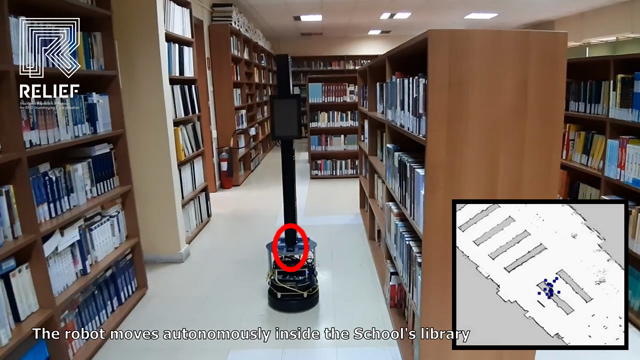
\includegraphics[height=101pt,width=180pt]{./figures/slides/ch3/relief_video_0_imgs/relief_video_0_023}
      \caption{\tiny  Εφαρμογή έργου RELIEF, βιβλιοθήκη ΤΗΜΜΥ, ΑΠΘ. \\ Πηγή: \url{https://relief.web.auth.gr/}}
    \end{figure}
  \end{minipage}
\end{minipage}
}

\note{\footnotesize
Η αυτόνομη πλοήγηση υποθέτει 5 προαπαιτούμενα.\\
Πρέπει να υπάρχει τουλάχιστον ένας εξωδεκτικός αισθητήρας, \\
ο χάρτης του περιβάλλοντος στο οποίο πλοηγείται το ρομπότ}

\end{frame}
